% !TEX TS-program = pdflatex
% !TEX encoding = UTF-8 Unicode

% This is a simple template for a LaTeX document using the "article" class.
% See "book", "report", "letter" for other types of document.

\documentclass[11pt]{article} % use larger type; default would be 10pt

\usepackage[T1]{fontenc}
\usepackage[utf8]{inputenc} % set input encoding (not needed with XeLaTeX)
\usepackage[ngerman]{babel}
\usepackage{marvosym}
\DeclareUnicodeCharacter{20AC}{\EUR}

%%% Examples of Article customizations
% These packages are optional, depending whether you want the features they provide.
% See the LaTeX Companion or other references for full information.

%%% PAGE DIMENSIONS
\usepackage{geometry} % to change the page dimensions
\geometry{a4paper} % or letterpaper (US) or a5paper or....
% \geometry{margin=2in} % for example, change the margins to 2 inches all round
% \geometry{landscape} % set up the page for landscape
%   read geometry.pdf for detailed page layout information

\usepackage{graphicx} % support the \includegraphics command and options

% \usepackage[parfill]{parskip} % Activate to begin paragraphs with an empty line rather than an indent

%%% PACKAGES
\usepackage{booktabs} % for much better looking tables
\usepackage{array} % for better arrays (eg matrices) in maths
\usepackage{paralist} % very flexible & customisable lists (eg. enumerate/itemize, etc.)
\usepackage{verbatim} % adds environment for commenting out blocks of text & for better verbatim
\usepackage{subfig} % make it possible to include more than one captioned figure/table in a single float
% These packages are all incorporated in the memoir class to one degree or another...

%%% HEADERS & FOOTERS
\usepackage{fancyhdr} % This should be set AFTER setting up the page geometry
\pagestyle{fancy} % options: empty , plain , fancy
\renewcommand{\headrulewidth}{0pt} % customise the layout...
\lhead{}\chead{}\rhead{}
\lfoot{}\cfoot{\thepage}\rfoot{}

%%% SECTION TITLE APPEARANCE
\usepackage{sectsty}
\allsectionsfont{\sffamily\mdseries\upshape} % (See the fntguide.pdf for font help)
% (This matches ConTeXt defaults)

%%% ToC (table of contents) APPEARANCE
\usepackage[nottoc,notlof,notlot]{tocbibind} % Put the bibliography in the ToC
\usepackage[titles,subfigure]{tocloft} % Alter the style of the Table of Contents
\renewcommand{\cftsecfont}{\rmfamily\mdseries\upshape}
\renewcommand{\cftsecpagefont}{\rmfamily\mdseries\upshape} % No bold!

%%% END Article customizations

%%% The "real" document content comes below...

\title{Handbuch „Cash Register“ \\ \large Ein einfaches RFID gestütztes Bezahlsystem mit Datenbankanbindung als geschlossenes System}
\author{Moritz Hilberg 733760 \and Lukas Köhler 734188}
%\date{} % Activate to display a given date or no date (if empty),
         % otherwise the current date is printed 

\begin{document}
\maketitle
\tableofcontents
\section{Installation und unterstützte Hardware}

-> welches BS
-> welches Reader-Bord
-> benötigte libs und packete (jSSC, sqlite3)
-> Erklärung config Datei

\section{Benutzerführung und Funktionen}
-> kurze Erklärung zu den Views

\begin{figure}[htb] \centering
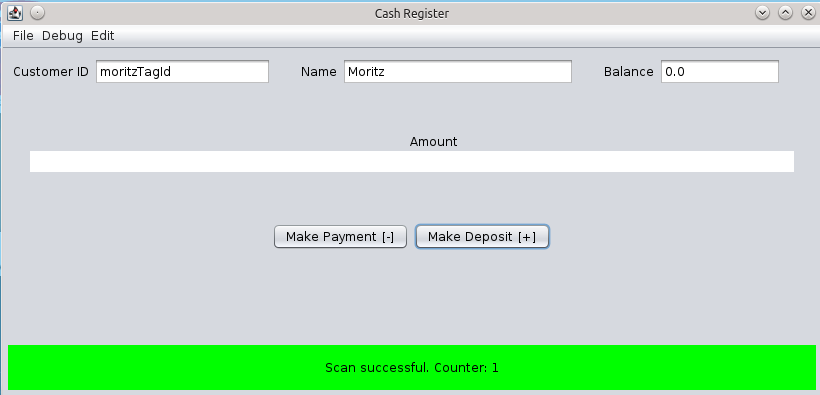
\includegraphics[height=5cm,keepaspectratio]{snapshot1.png}
\caption{}
\end{figure}

\begin{figure}[htb] \centering
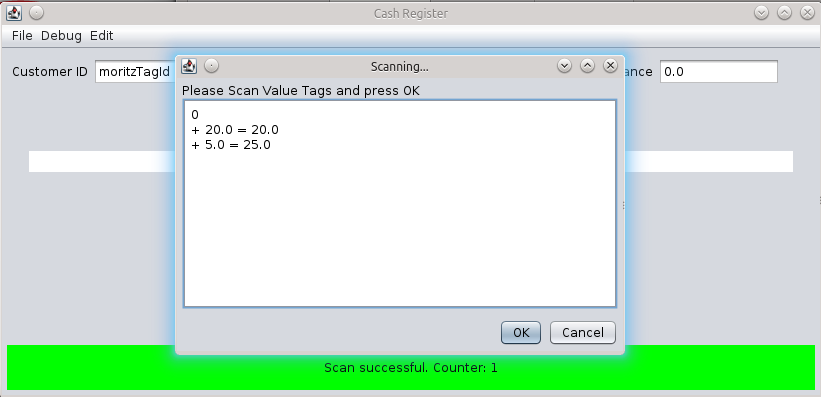
\includegraphics[height=5cm,keepaspectratio]{snapshot2.png}
\caption{}
\end{figure}

\begin{figure}[htb] \centering
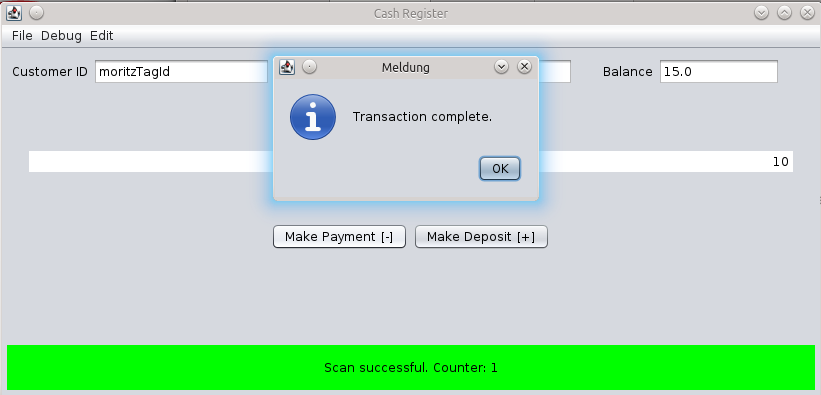
\includegraphics[height=5cm,keepaspectratio]{snapshot3.png}
\caption{}
\end{figure}

\begin{figure}[htb] \centering
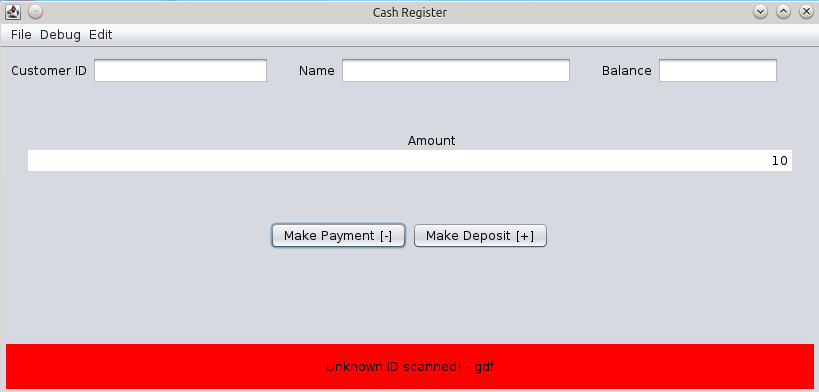
\includegraphics[height=5cm,keepaspectratio]{snapshot4.png}
\caption{}
\end{figure}

\begin{figure}[htb] \centering
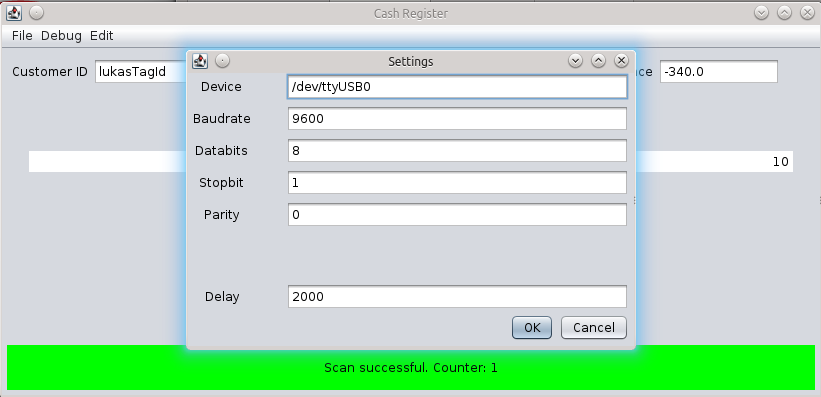
\includegraphics[height=5cm,keepaspectratio]{snapshot5.png}
\caption{}
\end{figure}


\section{Beschreibung der Realisierung mittels UML Klassendiagrammen}
-> kurz Ablauf der Kommunikation MVC erklären

\section{Anhang}
\begin{figure}[htb] \centering
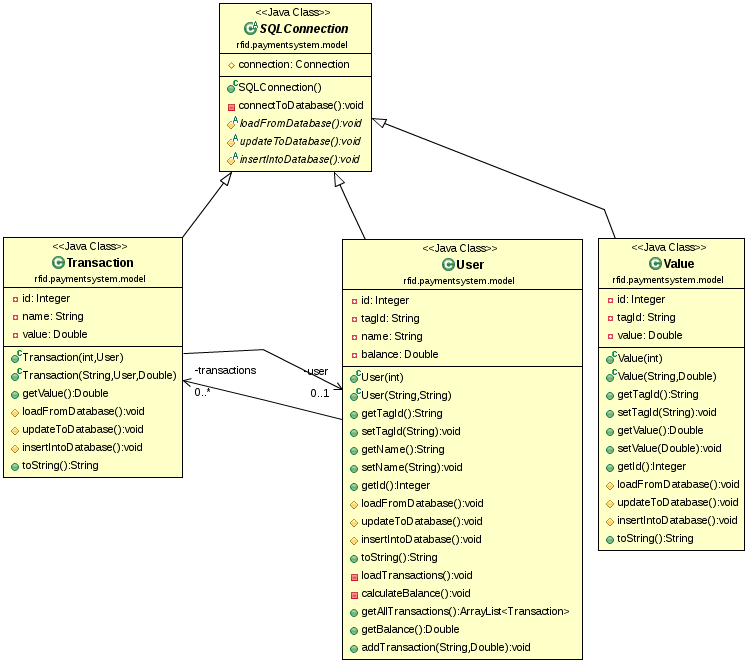
\includegraphics[width=\textwidth,keepaspectratio=true]{UML_Model.png}
\caption{MVC - Model}
\end{figure}
\begin{figure}[htb] \centering
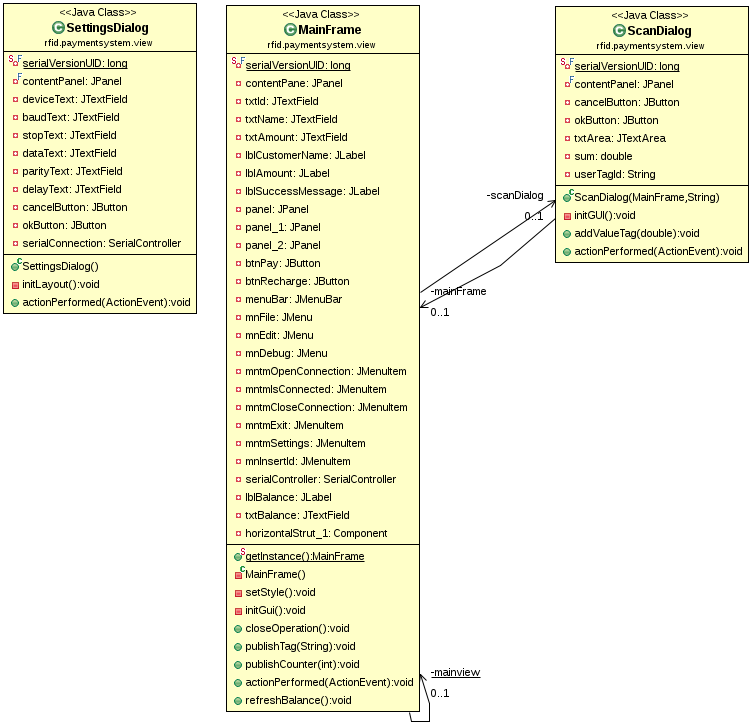
\includegraphics[width=\textwidth,keepaspectratio=true]{UML_View.png}
\caption{MVC - View}
\end{figure}
\begin{figure}[htb] \centering
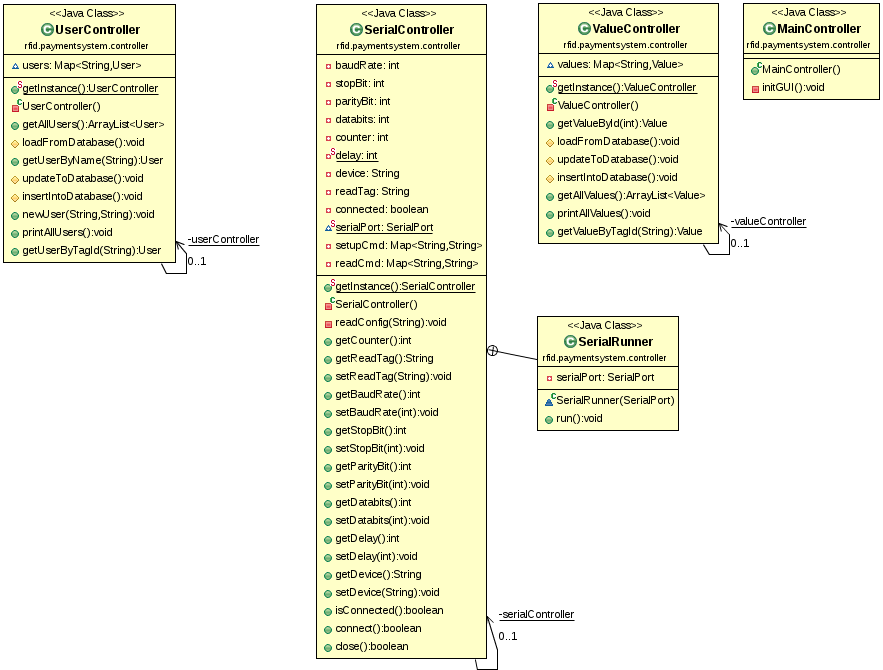
\includegraphics[width=\textwidth,keepaspectratio=true]{UML_Controller.png}
\caption{MVC - Controller}
\end{figure}

\end{document}
